\Tsec{Билет №19}

\begin{leftrules}
Вынужденное комбинационное рассеяние (ВКР). Роль спонтанного рассеяния. Основные характеристики излучения ВКР. Особенности энергообмена между волнами при ВКР.
\\ \phantom{42} \hfill \textit{лекция 11} 
\end{leftrules}



ВКР вызвано колебаниями молекул, то есть переменной поляризуемостью среды.

Возникают две новые линии излучения, отстоящие по частоте от основной на $\hbar \omega = E_{\text{кол}}$

Интенсивность не зависит от угла рассеяния, зависит от температуры.

\begin{equation}
    \frac{I_{\text{стокс}}}{I_{\text{антистокс}}} \gg \exp(-\frac{\hbar \omega}{k T})
\end{equation}

Основная и рассеянная волны складываются, итоговая интенсивность осциллирует на частоте молекулярных колебаний, что поддерживает возбуждение новых колебаний.

\begin{figure}[ht]
    \centering
    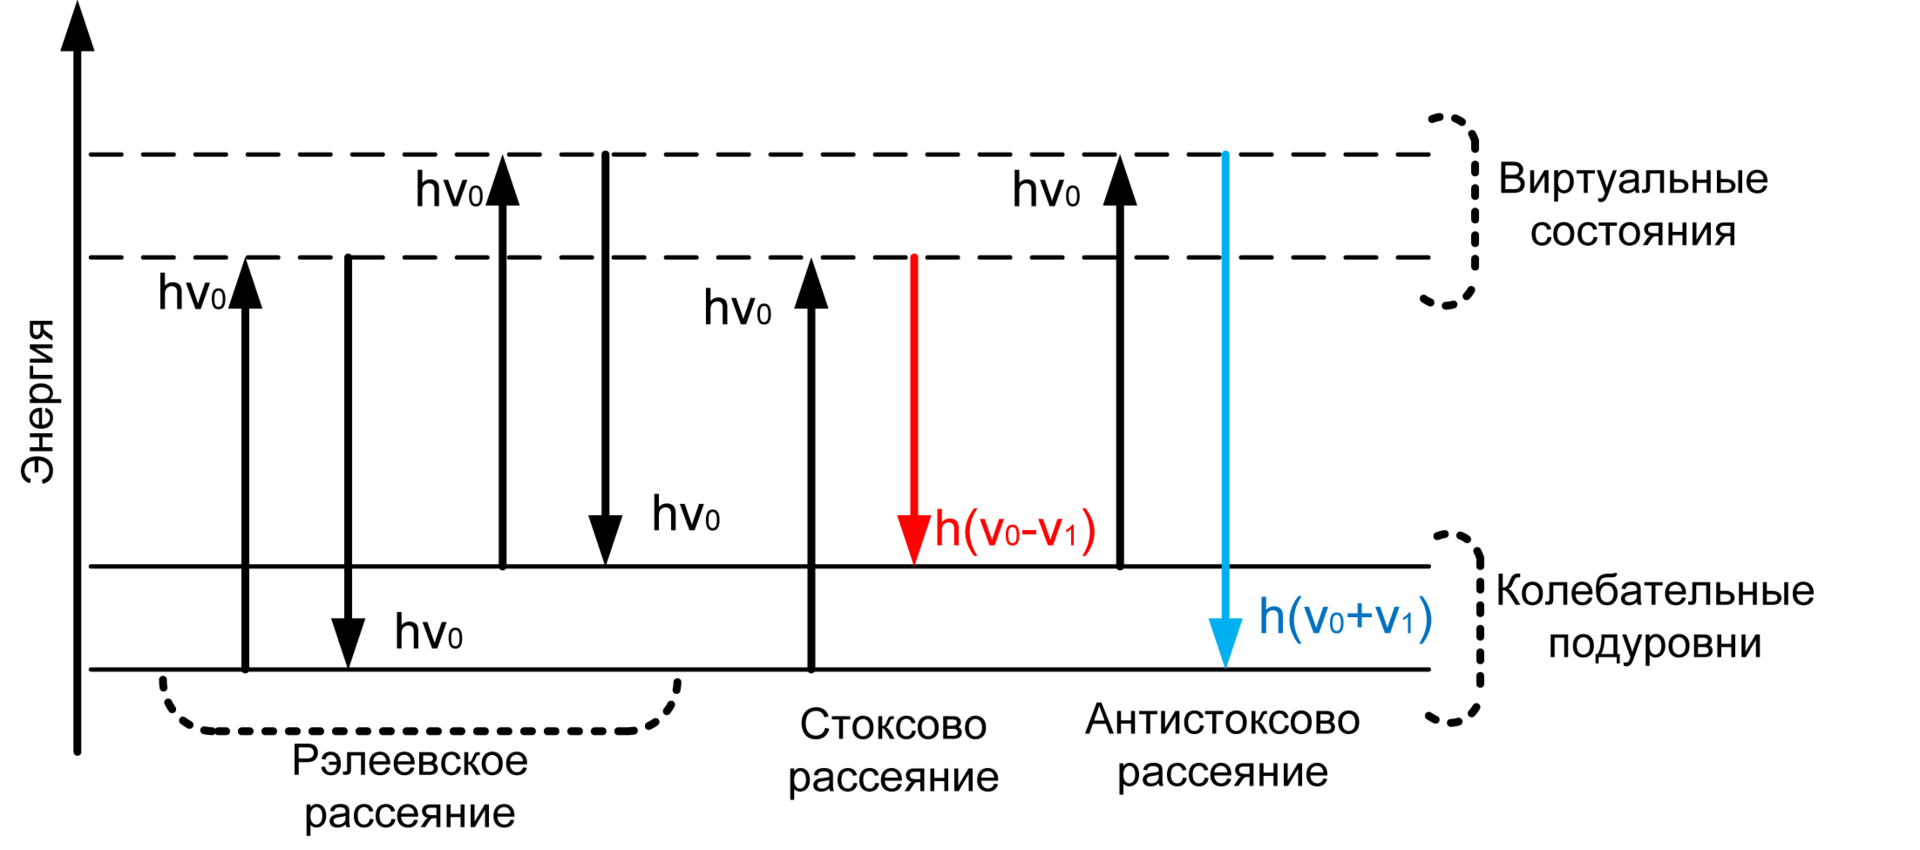
\includegraphics[width=0.6\textwidth]{figures/19-1.png}
    % \caption{19.}
    % \label{fig:my_label}
\end{figure}

Способ описания -- система с двумя уровнями энергии, для которой решается уравнение Шредингера.

Волна на стоксовой частоте усиливается, на антистоксовой ослабевает.
